\documentclass{beamer}
\usetheme{CambridgeUS}

\usepackage{amsmath}

\title{Do Taxes Impact Firm Location?}
\subtitle{A Panel Data Study of Matched County Pairs}
\author{Kevin D. Duncan}
\institute{Iowa State University}
\date{MSc Defense, June 29th 2015}

\begin{document}

\begin{frame}
\title{Do Taxes Impact Firm Entry on the Margin?}
\subtitle{A Panel Data Study of Matched County Pairs}
\author{Kevin D. Duncan}
\institute{Iowa State University}
\date{MSc Defense, July 29th 2015}
\maketitle
\end{frame}

\begin{frame}
\frametitle{Table of Contents}
\tableofcontents
\end{frame}

\begin{frame}
\section{Introduction \& Motivation}
\frametitle{Introduction}
Our paper studies the following two problems
\begin{itemize}
\item How do changes in tax and regulatory policy impact firm entry?
\item Do firms have preferences for government provided amenities?
\end{itemize}

This is motivated by the following problems:
\begin{itemize}
\item States and counties offer tax breaks and infrastructure as promises to bring in larger firms, but do small policy changes have benefits as well?
\item Does raising taxes to pay for various government services have distortionary effects?
\end{itemize}
We utilize both count data models and regression discontinuities around state borders to address this problem
\end{frame}

\begin{frame}
\section{Literature Review}
\frametitle{Literature Review}
\begin{itemize}
\item Empirical entry studies of firms (Gabe and Bell (2004), Brulhart et al (2012)) include Tiebout-style (1956) considerations into count data models, which state individuals sort into counties based off of prices and public goods. Instead they look at taxes and public expenditures w.r.t. firm entry.
\begin{itemize}
\item Gabe and Bell show that increasing taxes to pay for education seems to have no adverse effect on firm entry.
\item Brulhart et al shows no significant impact of spending on firm start up rates. But that higher agglomeration will weaken negative impacts of taxes.
\end{itemize}
\item Regression discontinuities around state borders have been used to test the relative growth in employment (Holmes (1998), Dube et al (2010)) as well as firm location (Rohlin (2011)) using minimum wages and right to work status.
\end{itemize}
\end{frame}

\begin{frame}
\section{Theory}
\frametitle{Theory Pt I}
\begin{itemize}
\item  Wages and capital costs are adjusted to local tax and location specific measures affecting firm level productivity. If markets are competitive firms will make zero economic profit in the long run, but demand or policy shocks leave short term profits.
\item If a regime changes its taxes over time, higher production costs and lower profits exist in that county, and that market will deter a relative amount of firms from entering as firms enter and bid up prices on the other side.
\item Firms make decisions based on information from the previous year, as governments might concurrently change policy along with market entry. 
\end{itemize}
\end{frame}

\begin{frame}
\frametitle{Theory Pt II}
\begin{itemize}
\item Assumption 1: Period specific profit functions can be represented by a linear function;
\begin{equation} \label{profit}
\pi_{i,j,t} =  X_{i,j,t-1}\beta+\epsilon_{i,j,t}
\end{equation}
\item $i$ indexes location, $j$ indexes regime, and $t$ is time period. $\beta$ is assumed to be time invariant, and shared across all regimes.
\item $X_{i,t,t-1}$ is a $1 \times K$ row vector, and $\beta$ is a $K \times 1$ column vector.
\end{itemize}
\end{frame}

\begin{frame}
\frametitle{Theory Pt III}
Let us focus on an interval $[-1,1]$, where if $i \in [-1,0)$, $i$ is in regime $A$, and if $i \in [0,1]$, $i$ is in regime $B$. Then, contingent on firms first choosing to move into one of two locations $y \in [-1,0)$ and $\hat y \in [0,1]$ then the choice of a new entrant to prefer $y$ over $\hat y$ is;

$$ E[\pi_{y,A,t}-\pi_{\hat y,B,t}|X_{y,A,t-1},X_{\hat y,B,t-1}] = (X_{y,A,t-1}-X_{\hat y,B,t-1})\beta > 0 $$

Assumption 2: We can partition $X_{i,j,t-1}$, such that $X_{i,j,t-1}= [X_{i,t-1} \quad X_{j,t-1}]$ is a $1 \times K_{i} + K_{j}$ matrix and $\beta = [\beta_{i} \quad \beta_{j}]'$ is a $K_{i} + K_{j} \times 1$ matrix.

Assumption 3: $X_{i,t}$ is continuous locally around the discontinuity

Assumption 4: $X_{j,t} \neq X_{j',t}, \quad \forall j' \neq j$

Then we see that as $y,\hat y \to 0$ the choice becomes;
$$ E[\pi_{y,A,t}-\pi_{\hat y,B,t}|X_{y,A,t-1},X_{\hat y,B,t-1}] = (X_{A,t-1}-X_{B,t-1})\beta_{j} > 0$$
\end{frame}


\begin{frame}
\section{Empirical Design \& Results}
\frametitle{Empirical Outline}
Our empirical framework is developed as follows:
\begin{itemize}
\item Discussion of data
\item Count data models
\item Issues in count data models
\item Regression discontinuity technique
\item Robustness checks: 
\begin{itemize}
\item Test if coefficients are the same on either side of the border
\item Test if coefficients are stable across time
\item Test interaction terms between taxes and government expenditures
\end{itemize}
\end{itemize}
\end{frame}

\begin{frame}
\frametitle{Data}
\begin{itemize}
\item Total number of firm start ups in every continental US county
\item Seven different state top marginal tax rates
\begin{itemize}
\item property, income, capital gains, sales, corporate, workers compensation, unemployment insurance
\end{itemize}
\item State right to work status and minimum wage
\item Log state expenditures per capita on education, highways, and welfare
\item Scaled county geographic amenities
\item Additional Controls: County level real fuel prices, pct with high school education, population density, pct unionized, pct manufacturing
\end{itemize}
\end{frame}

\begin{frame}
\subsection{Count Data Models}
\frametitle{Count Data Models}
The firms entry profit is claimed to be;
$$\pi_{i,j,t} = X_{i,t}\beta_{i}+X_{j,t}\beta+\epsilon_{i,j,t}$$
Conditional logit estimation entry under this profit function morphs into Poisson models of the number of firm entry under as long as choice-specific parameters are shared between all firms (Guimaraes, Figueirido, and Woodward (2003)). We estimate
\begin{equation} \label{pois}
ln(E[n_{ijt}|X_{j,t-1}]) = X_{j,t-1}\beta
\end{equation}
$$\implies E[n_{ijt}|X_{j,t-1}] = \exp(X_{j,t-1}\beta)$$

We further estimate both a negative binomial and normal regression utilizing (\ref{pois}).
\end{frame}

\begin{frame}
\frametitle{CDM Results}
\begin{itemize}
\item Poisson: property, income, corporate, workers comp tax rates and welfare spending per cap were all positive and statistically significantly tied to firm start up rates. Capital gains, sales, and unemployment insurance tax rates as well as education and hwy spending per capita were negative and statistically significantly related to firm start up rates.
\item Negative Binomial \& Normal: All taxes besides for corporate tax rates became negative and statistically significantly different from zero in their impacts on firm start up rates. Right to work status lowers firm start up rates, and minimum wage increases it. Similar to Poisson, education and highway spending per capita are negative, while welfare spending per capita is positive.
\end{itemize}
\end{frame}

\begin{frame}
\frametitle{Issues with Count Data Models}
\begin{itemize}
\item The full model should be
\begin{equation}
ln(E[n_{i,j,t}|X_{i,j,t}]) = X_{i,t-1}\beta_{i}+X_{j,t-1}\beta_{j}+\epsilon_{i,j,t}
\end{equation}
\item We only estimated
$$ln(n_{i,j,t}) = X_{j,t-1}\beta_{j}+v_{i,j,t}$$
$$v_{i,j,t} = X_{i,t}\beta_{i}+\epsilon_{i,j,t}$$
\item For Poisson distribution, we need
$$E[v_{i,j,t}] = 0 \implies E[X_{i,t}\beta_{i}] = 0$$
\item We also need $E[X_{j}'v_{i,j}] = 0$ for method of moments estimation
\item As a result of this our count data models may not be properly identified by either omitted variable bias or unobserved location specific heterogeneity.
\end{itemize}
\end{frame}

\begin{frame}
\subsection{Regression Discontinuity Design}
\frametitle{Regression Discontinuity Design pt I}
By matching county pairs that are close together we are able to properly account for location specific terms
\begin{itemize}
\item  Proxy distance from the border by matching two counties on either side of a state border, denoting them $sub$ and $nbr$ arbitrarily.
\item From our theory we show how the location effect drops out as we approach the border
\item Controls for the unobserved local effect heterogeneity
\item We estimate for each pair of matched counties, indexed by $j$
\end{itemize}

\begin{equation} \label{pols}
\ddot{ln(n_{j,t})} = \ddot x_{j,t-1}\beta_{j} + \ddot \epsilon_{j,t}
\end{equation}
 $$\ddot{ln(n_{j,t})} = ln(n_{sub,t})-ln(n_{nbr,t})$$
 $$\ddot x_{j,t-1} = x_{sub,t-1}-x_{nbr,t-1}$$
 $$\ddot \epsilon_{j,t} = \epsilon_{sub,t}-\epsilon_{nbr,t}$$
\end{frame}

\begin{frame}
\frametitle{Regression Discontinuity Design pt II}
\begin{itemize}
\item We have $G$ state-pairs, which are borders where two states meet.
\item We see each state-pair $N_{g}$ times each year, once for each matched county-pairs
\item and we have $T$ time periods
\item Assuming from (\ref{pols}) 
\begin{equation}\label{moment}
E[\ddot X_{j}'\ddot \epsilon_{j}] = 0
\end{equation}
we get the POLS estimator
\begin{equation}\label{polsest}
\hat \beta = \left(\frac{1}{N}\sum_{t=1}^{T}\sum_{g=1}^{G}\sum_{i=1}^{N_{G}}\ddot x_{g,t-1}'\ddot x_{g,t-1}\right)^{-1}\left(\frac{1}{N}\sum_{t=1}^{T}\sum_{g=1}^{G}\sum_{i=1}^{N_{G}}\ddot x_{g,t-1}'\ddot ln(n_{i,g,t})\right)
\end{equation}
\begin{equation}\label{norm}
N = T(\sum_{g=1}^{G}N_{G})
\end{equation}
\end{itemize}
\end{frame}

\begin{frame}
\frametitle{Regression Discontinuity Design pt III}
\begin{itemize}
\item For (\ref{moment}) we need that states do not change policy with respect to firm entry. There seems no \textit{a priori} reason to assume that governments care more about one border pair over any other, unless they may be systemically having problems with all of their neighbors at once.
\item We might have a border-pair specific effect remaining in $\epsilon_{i,j,t}$, even if (\ref{moment}) holds. Thus we use clustered standard errors. 
\end{itemize}
\end{frame}


\begin{frame}
\frametitle{RD Results}
\begin{table}[!htbp] \centering 
{\tiny\renewcommand{\arraystretch}{.8}
\resizebox{!}{.35\paperheight}{%
\begin{tabular}{@{\extracolsep{5pt}}lcccc} 
\\[-1.8ex]\hline 
\hline \\[-1.8ex] 
 & \multicolumn{4}{c}{\textit{Dependent variable:}} \\ 
\cline{2-5} 
\\[-1.8ex] & \multicolumn{2}{c}{births\_diff } & \multicolumn{2}{c}{births\_ratio } \\ 
\\[-1.8ex] & (1) & (2) & (3) & (4)\\ 
\hline \\[-1.8ex] 
 ptax\_ratio\_L1 & $-$124.433$^{**}$ & $-$125.628$^{**}$ & $-$0.444$^{***}$ & $-$0.456$^{***}$ \\ 
  & (59.341) & (58.776) & (0.152) & (0.152) \\ 
  & & & & \\ 
 inctax\_ratio\_L1 & $-$8.969 & $-$8.294 & $-$0.077$^{***}$ & $-$0.077$^{***}$ \\ 
  & (11.515) & (11.468) & (0.026) & (0.026) \\ 
  & & & & \\ 
 capgntax\_ratio\_L1 & 4.853 & 4.800 & 0.003 & 0.002 \\ 
  & (8.539) & (8.274) & (0.023) & (0.023) \\ 
  & & & & \\ 
 stax\_ratio\_L1 & $-$11.218 & $-$10.825 & $-$0.099$^{***}$ & $-$0.100$^{***}$ \\ 
  & (13.724) & (13.477) & (0.028) & (0.028) \\ 
  & & & & \\ 
 corptax\_ratio\_L1 & $-$1.603 & $-$2.314 & 0.021 & 0.020 \\ 
  & (6.330) & (6.459) & (0.018) & (0.018) \\ 
  & & & & \\ 
 wctax\_ratio\_L1 & 103.002 & 102.075 & 0.088 & 0.094 \\ 
  & (67.313) & (67.289) & (0.119) & (0.119) \\ 
  & & & & \\ 
 uitax\_ratio\_L1 & 1,581.092 & 1,622.265 & 0.972 & 1.179 \\ 
  & (1,586.044) & (1,561.253) & (3.594) & (3.594) \\ 
  & & & & \\ 
 minwage\_L1\_ratio & 11.805 & 11.280 & $-$0.062 & $-$0.055 \\ 
  & (27.104) & (26.439) & (0.073) & (0.073) \\ 
  & & & & \\ 
 rtw\_L1\_ratio & 110.586$^{**}$ & 113.241$^{**}$ & 0.067 & 0.080 \\ 
  & (52.663) & (52.012) & (0.135) & (0.135) \\ 
  & & & & \\ 
 educ\_ratio\_L1 & $-$189.173$^{*}$ & $-$190.860$^{*}$ & $-$0.154 & $-$0.154 \\ 
  & (102.900) & (103.087) & (0.184) & (0.184) \\ 
  & & & & \\ 
 hwy\_ratio\_L1 & 12.375 & 13.592 & 0.146 & 0.135 \\ 
  & (67.477) & (66.531) & (0.129) & (0.129) \\ 
  & & & & \\ 
 welfare\_ratio\_L1 & 40.601 & 40.596 & 0.409$^{*}$ & 0.420$^{*}$ \\ 
  & (101.069) & (99.934) & (0.235) & (0.235) \\ 
  & & & & \\ 
  amenities & yes & no & yes & no \\
\hline \\[-1.8ex] 
\hline 
\hline \\[-1.8ex] 
\textit{Note:}  & \multicolumn{4}{r}{$^{*}$p$<$0.1; $^{**}$p$<$0.05; $^{***}$p$<$0.01} \\ 
\end{tabular}}} 
\end{table}
Controls drop out besides for real fuel price, which has a positive and strongly significant impact on firm start ups.
\end{frame}


\begin{frame}
\subsection{Sensitivity Tests}
\frametitle{Sensitivity Tests Pt I}
\begin{itemize}
\item We tested whether or not it was reasonable to believe that coefficients were the same across borders, which passed a series of F tests besides for workers compensation.
$$\ddot{ln(n_{j,t})} = X_{A,t-1}\beta_{A,j}+X_{B,t-1}\beta_{B,j} + \epsilon_{t}'$$ 
\begin{itemize}
\item Coefficients appeared to be equal and opposite, i.e. $\beta_{A,j} = - \beta_{B,j}$ as is predicted by our later model
\item Workers compensation tax was the one variable that was rejected at the 5\% level.
\end{itemize}
\end{itemize}
\end{frame}

\begin{frame}
\frametitle{Sensitivity Tests Pt II}
\begin{itemize}
\item We tested stability of coefficients across all 10 years in our sample
$$\ddot{ln(n_{j,t})} = \ddot X_{j,t-1}\beta_{j,t} + \epsilon_{t}': t = 1999,...,2008$$ 
\begin{itemize}
\item Property and Sales taxes remain about the same significance and sign across all 10 years. Income taxes moves from being insignificant to significant and negative as we move to more current years. Some highway and welfare expenditure variables are positive significant in the early years of our sample, but drop out in later ones. 
\end{itemize}
\end{itemize}
\end{frame}


\begin{frame}
\frametitle{Sensitivity Tests Pt III}
\begin{itemize}
\item tested interaction terms between a subset of taxes and government expenditures per capita
\begin{itemize}
\item For each tax $\tau_{i}$ and expenditure $exp_{j}$ calculated values by
\begin{equation}
\tau_{i}\_exp_{j} = \tau_{i,sub}exp_{j,sub}-\tau_{i,nbr}exp_{j,nbr}
\end{equation}
\item Only property taxes remained negative and significant with a coefficient greater than 1!
\item After doing joint tests of significance, property taxes and their interaction terms were significant from zero at the 1\% level
\item Marginal effects
\begin{itemize}
\item property taxes \& highway: -1.13
\item property taxes \& education: -.9
\item property taxes \& welfare: -.74
\end{itemize}
\end{itemize}
\end{itemize}
\end{frame}

\begin{frame}
\section{Analysis}
\frametitle{Some Comparisons}
We calculate the weighted tax differential. This is taken by multiplying our estimates for the impacts of taxes on firm start up rates. We then take the absolute value of this, to get an idea on the distribution of tax differentials imposed on the borders around states.
\begin{figure}
\centering
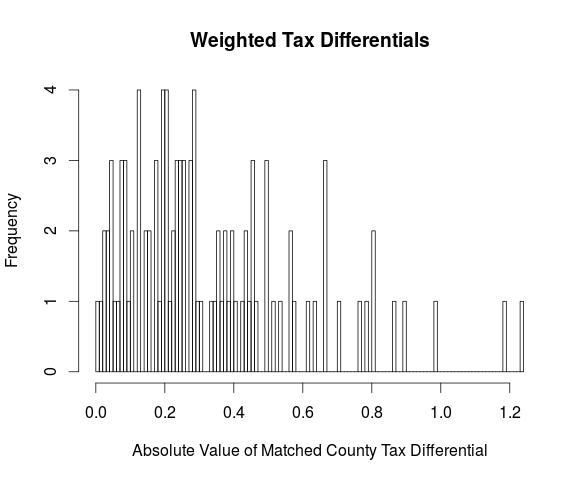
\includegraphics[scale=0.35]{taxdiff}
\end{figure}
\end{frame}

\begin{frame}
\frametitle{Some Comparisons Pt II}
Finally, we can rank average difference in firm start up rates and tax differential. Surprisingly we see that in the top 10 difference in mean start up rates along a state border, most of them share the same sign as the tax differential. Overall throughout our RD designs though, we find relatively low $R^{2}$ values.


\begin{table}[h]
\centering
\caption{Mean Firm Start Ups v Weighted Tax Differential}
{\tiny\renewcommand{\arraystretch}{.8}
\resizebox{\textwidth}{!}{%
\label{my-label}
\begin{tabular}{llll}
\hline \\[-1.8ex] 
Mean Firm Starts up & State Pair                      & Start up Favors & Tax Differential Favors \\
\hline \\[-1.8ex] 
1.642965            & Oklahoma - Texas                & Texas           & Oklahoma \\
1.621283            & New Mexico - Texas              & New Mexico      & New Mexico \\
1.548548            & Illinois - Missouri             & Missouri        & Missouri \\
1.546172            & Alabama - Georgia               & Alabama         & Alabama \\
1.435885            & California - Nevada             & Nevada          & Nevada \\
1.307654            & Indiana - Kentucky              & Kentucky        & Kentucky \\ 
1.257129            & North Carolina - South Carolina & South Carolina  & South Carolina \\
1.251866            & Oregon - Washington             & Oregon          & Oregon \\
1.233235            & North Carolina - Virginia       & Virginia        & Virginia \\
1.208313            & North Carolina - West Virginia  & North Carolina  & West Virginia \\
\hline
\end{tabular}}}
\end{table}

\end{frame}

\begin{frame}
\section{Conclusion}
\frametitle{Conclusion}
Going back to our original two research questions, we see that:
\begin{itemize}
\item Property, sales, and income taxes across most specifications besides for our interaction term regressions. 
\item Property tax rates have a relatively high elasticity, where a 1\% increase in relative property tax rates corresponds to a 0.49\% decrease in relative firm start up rates. This is stable and common across all our RD estimates
\item Sales tax rates have a lower elastcitiy, where a 1\% increase in relative sales tax rates corresponds to a 0.1\% decrease in relative firm start up rates.
\item This may be due to many firms being small, and so individuals on one side of the border (with preferential government expenditures) can start up a business in the neighboring county
\item Government expenditures on infrastructure, welfare, and education does not seem to impact firm start up rates

\end{itemize}
\end{frame}

\begin{frame}
\frametitle{Future Work or Extensions}
\begin{itemize}
\item Create data set over all counties in the US from 1999-2008 and re-run count data models
\begin{itemize}
\item Can we find ways to proxy or estimate location specific heterogeneity better? Calculating agglomeration figures for every county as a first attempt
\end{itemize}
\item Testing coefficients as we get further away from the border (match counties on opposite ends of the state, test for state fixed effects, etc)
\item Run estimator over sub samples of counties of different sizes
\item Can we optimizing estimator to account for number of observations seen?
\end{itemize}
\end{frame}

\begin{frame}
\begin{centering}
\huge{Thank you for your time!}
\end{centering}
\end{frame}
\end{document}